% !Mode:: "TeX:UTF-8"
\documentclass[12pt,a4paper]{article}

%%%%%%%%------------------------------------------------------------------------
%%%% 日常所用宏包

%% 控制页边距
% 如果是beamer文档类, 则不用geometry
\makeatletter
\@ifclassloaded{beamer}{}{\usepackage[top=2.5cm, bottom=2.5cm, left=2.5cm, right=2.5cm]{geometry}}
\makeatother

%% 控制项目列表
\usepackage{enumerate}

%% 多栏显示
\usepackage{multicol}

%% 算法环境
\usepackage{algorithm}  
\usepackage{algorithmic} 
\usepackage{float} 

%% 网址引用
\usepackage{url}

%% 控制矩阵行距
\renewcommand\arraystretch{1.4}

%% hyperref宏包,生成可定位点击的超链接,并且会生成pdf书签
\makeatletter
\@ifclassloaded{beamer}{
\usepackage{hyperref}
\usepackage{ragged2e} % 对齐
}{
\usepackage[%
    pdfstartview=FitH,%
    CJKbookmarks=true,%
    bookmarks=true,%
    bookmarksnumbered=true,%
    bookmarksopen=true,%
    colorlinks=true,%
    citecolor=blue,%
    linkcolor=blue,%
    anchorcolor=green,%
    urlcolor=blue%
]{hyperref}
}
\makeatother



\makeatletter % 如果是 beamer 不需要下面两个包
\@ifclassloaded{beamer}{
\mode<presentation>
{
} 
}{
%% 控制标题
\usepackage{titlesec}
%% 控制目录
\usepackage{titletoc}
}
\makeatother

%% 控制表格样式
\usepackage{booktabs}

%% 控制字体大小
\usepackage{type1cm}

%% 首行缩进,用\noindent取消某段缩进
\usepackage{indentfirst}

%% 支持彩色文本、底色、文本框等
\usepackage{color,xcolor}

%% AMS LaTeX宏包: http://zzg34b.w3.c361.com/package/maths.htm#amssymb
\usepackage{amsmath,amssymb}
%% 多个图形并排
\usepackage{subfig}
%%%% 基本插图方法
%% 图形宏包
\usepackage{graphicx}
\newcommand{\red}[1]{\textcolor{red}{#1}}
\newcommand{\blue}[1]{\structure{#1}}
\newcommand{\brown}[1]{\textcolor{brown}{#1}}
\newcommand{\green}[1]{\textcolor{green}{#1}}


%%%% 基本插图方法结束

%%%% pgf/tikz绘图宏包设置
\usepackage{pgf,tikz}
\usetikzlibrary{shapes,automata,snakes,backgrounds,arrows}
\usetikzlibrary{mindmap}
%% 可以直接在latex文档中使用graphviz/dot语言,
%% 也可以用dot2tex工具将dot文件转换成tex文件再include进来
%% \usepackage[shell,pgf,outputdir={docgraphs/}]{dot2texi}
%%%% pgf/tikz设置结束


\makeatletter % 如果是 beamer 不需要下面两个包
\@ifclassloaded{beamer}{

}{
%%%% fancyhdr设置页眉页脚
%% 页眉页脚宏包
\usepackage{fancyhdr}
%% 页眉页脚风格
\pagestyle{plain}
}

%% 有时会出现\headheight too small的warning
\setlength{\headheight}{15pt}

%% 清空当前页眉页脚的默认设置
%\fancyhf{}
%%%% fancyhdr设置结束


\makeatletter % 对 beamer 要重新设置
\@ifclassloaded{beamer}{

}{
%%%% 设置listings宏包用来粘贴源代码
%% 方便粘贴源代码,部分代码高亮功能
\usepackage{listings}

%% 设置listings宏包的一些全局样式
%% 参考http://hi.baidu.com/shawpinlee/blog/item/9ec431cbae28e41cbe09e6e4.html
\lstset{
showstringspaces=false,              %% 设定是否显示代码之间的空格符号
numbers=left,                        %% 在左边显示行号
numberstyle=\tiny,                   %% 设定行号字体的大小
basicstyle=\footnotesize,                    %% 设定字体大小\tiny, \small, \Large等等
keywordstyle=\color{blue!70}, commentstyle=\color{red!50!green!50!blue!50},
                                     %% 关键字高亮
frame=shadowbox,                     %% 给代码加框
rulesepcolor=\color{red!20!green!20!blue!20},
escapechar=`,                        %% 中文逃逸字符,用于中英混排
xleftmargin=2em,xrightmargin=2em, aboveskip=1em,
breaklines,                          %% 这条命令可以让LaTeX自动将长的代码行换行排版
extendedchars=false                  %% 这一条命令可以解决代码跨页时,章节标题,页眉等汉字不显示的问题
}}
\makeatother
%%%% listings宏包设置结束


%%%% 附录设置
\makeatletter % 对 beamer 要重新设置
\@ifclassloaded{beamer}{

}{
\usepackage[title,titletoc,header]{appendix}
}
\makeatother
%%%% 附录设置结束


%%%% 日常宏包设置结束
%%%%%%%%------------------------------------------------------------------------


%%%%%%%%------------------------------------------------------------------------
%%%% 英文字体设置结束
%% 这里可以加入自己的英文字体设置
%%%%%%%%------------------------------------------------------------------------

%%%%%%%%------------------------------------------------------------------------
%%%% 设置常用字体字号,与MS Word相对应

%% 一号, 1.4倍行距
\newcommand{\yihao}{\fontsize{26pt}{36pt}\selectfont}
%% 二号, 1.25倍行距
\newcommand{\erhao}{\fontsize{22pt}{28pt}\selectfont}
%% 小二, 单倍行距
\newcommand{\xiaoer}{\fontsize{18pt}{18pt}\selectfont}
%% 三号, 1.5倍行距
\newcommand{\sanhao}{\fontsize{16pt}{24pt}\selectfont}
%% 小三, 1.5倍行距
\newcommand{\xiaosan}{\fontsize{15pt}{22pt}\selectfont}
%% 四号, 1.5倍行距
\newcommand{\sihao}{\fontsize{14pt}{21pt}\selectfont}
%% 半四, 1.5倍行距
\newcommand{\bansi}{\fontsize{13pt}{19.5pt}\selectfont}
%% 小四, 1.5倍行距
\newcommand{\xiaosi}{\fontsize{12pt}{18pt}\selectfont}
%% 大五, 单倍行距
\newcommand{\dawu}{\fontsize{11pt}{11pt}\selectfont}
%% 五号, 单倍行距
\newcommand{\wuhao}{\fontsize{10.5pt}{10.5pt}\selectfont}
%%%%%%%%------------------------------------------------------------------------


%% 设定段间距
\setlength{\parskip}{0.5\baselineskip}

%% 设定行距
\linespread{1}


%% 设定正文字体大小
% \renewcommand{\normalsize}{\sihao}

%制作水印
\RequirePackage{draftcopy}
\draftcopyName{XTUMESH}{100}
\draftcopySetGrey{0.90}
\draftcopyPageTransform{40 rotate}
\draftcopyPageX{350}
\draftcopyPageY{80}

%%%% 个性设置结束
%%%%%%%%------------------------------------------------------------------------


%%%%%%%%------------------------------------------------------------------------
%%%% bibtex设置

%% 设定参考文献显示风格
% 下面是几种常见的样式
% * plain: 按字母的顺序排列,比较次序为作者、年度和标题
% * unsrt: 样式同plain,只是按照引用的先后排序
% * alpha: 用作者名首字母+年份后两位作标号,以字母顺序排序
% * abbrv: 类似plain,将月份全拼改为缩写,更显紧凑
% * apalike: 美国心理学学会期刊样式, 引用样式 [Tailper and Zang, 2006]

\makeatletter
\@ifclassloaded{beamer}{
\bibliographystyle{apalike}
}{
\bibliographystyle{unsrt}
}
\makeatother


%%%% bibtex设置结束
%%%%%%%%------------------------------------------------------------------------

%%%%%%%%------------------------------------------------------------------------
%%%% xeCJK相关宏包

\usepackage{xltxtra,fontspec,xunicode}
\usepackage[slantfont, boldfont]{xeCJK} 

%% 针对中文进行断行
\XeTeXlinebreaklocale "zh"             

%% 给予TeX断行一定自由度
\XeTeXlinebreakskip = 0pt plus 1pt minus 0.1pt

%%%% xeCJK设置结束                                       
%%%%%%%%------------------------------------------------------------------------

%%%%%%%%------------------------------------------------------------------------
%%%% xeCJK字体设置

%% 设置中文标点样式,支持quanjiao、banjiao、kaiming等多种方式
\punctstyle{kaiming}                                        
                                                     
%% 设置缺省中文字体
\setCJKmainfont[BoldFont={Adobe Heiti Std}, ItalicFont={Adobe Kaiti Std}]{Adobe Song Std}   
%% 设置中文无衬线字体
\setCJKsansfont[BoldFont={Adobe Heiti Std}]{Adobe Kaiti Std}  
%% 设置等宽字体
\setCJKmonofont{Adobe Heiti Std}                            

%% 英文衬线字体
\setmainfont{DejaVu Serif}                                  
%% 英文等宽字体
\setmonofont{DejaVu Sans Mono}                              
%% 英文无衬线字体
\setsansfont{DejaVu Sans}                                   

%% 定义新字体
\setCJKfamilyfont{song}{Adobe Song Std}                     
\setCJKfamilyfont{kai}{Adobe Kaiti Std}
\setCJKfamilyfont{hei}{Adobe Heiti Std}
\setCJKfamilyfont{fangsong}{Adobe Fangsong Std}
\setCJKfamilyfont{lisu}{LiSu}
\setCJKfamilyfont{youyuan}{YouYuan}

%% 自定义宋体
\newcommand{\song}{\CJKfamily{song}}                       
%% 自定义楷体
\newcommand{\kai}{\CJKfamily{kai}}                         
%% 自定义黑体
\newcommand{\hei}{\CJKfamily{hei}}                         
%% 自定义仿宋体
\newcommand{\fangsong}{\CJKfamily{fangsong}}               
%% 自定义隶书
\newcommand{\lisu}{\CJKfamily{lisu}}                       
%% 自定义幼圆
\newcommand{\youyuan}{\CJKfamily{youyuan}}                 

%%%% xeCJK字体设置结束
%%%%%%%%------------------------------------------------------------------------

%%%%%%%%------------------------------------------------------------------------
%%%% 一些关于中文文档的重定义
\newcommand{\chntoday}{\number\year\,年\,\number\month\,月\,\number\day\,日}
%% 数学公式定理的重定义

%% 中文破折号,据说来自清华模板
\newcommand{\pozhehao}{\kern0.3ex\rule[0.8ex]{2em}{0.1ex}\kern0.3ex}

\newtheorem{example}{例}                                   
\newtheorem{theorem}{定理}[section]                         
\newtheorem{definition}{定义}
\newtheorem{axiom}{公理}
\newtheorem{property}{性质}
\newtheorem{proposition}{命题}
\newtheorem{lemma}{引理}
\newtheorem{corollary}{推论}
\newtheorem{remark}{注解}
\newtheorem{condition}{条件}
\newtheorem{conclusion}{结论}
\newtheorem{assumption}{假设}

\makeatletter %
\@ifclassloaded{beamer}{

}{
%% 章节等名称重定义
\renewcommand{\contentsname}{目录}     
\renewcommand{\indexname}{索引}
\renewcommand{\listfigurename}{插图目录}
\renewcommand{\listtablename}{表格目录}
\renewcommand{\appendixname}{附录}
\renewcommand{\appendixpagename}{附录}
\renewcommand{\appendixtocname}{附录}
%% 设置chapter、section与subsection的格式
\titleformat{\chapter}{\centering\huge}{第\thechapter{}章}{1em}{\textbf}
\titleformat{\section}{\centering\sihao}{\thesection}{1em}{\textbf}
\titleformat{\subsection}{\xiaosi}{\thesubsection}{1em}{\textbf}
\titleformat{\subsubsection}{\xiaosi}{\thesubsubsection}{1em}{\textbf}

\@ifclassloaded{book}{

}{
\renewcommand{\abstractname}{摘要}
}
}
\makeatother

\renewcommand{\figurename}{图}
\renewcommand{\tablename}{表}

\makeatletter
\@ifclassloaded{book}{
\renewcommand{\bibname}{参考文献}
}{
\renewcommand{\refname}{参考文献} 
}
\makeatother

\floatname{algorithm}{算法}
\renewcommand{\algorithmicrequire}{\textbf{输入:}}
\renewcommand{\algorithmicensure}{\textbf{输出:}}

%%%% 中文重定义结束
%%%%%%%%------------------------------------------------------------------------


\title{光滑有限元法(S-FEM):理想解的数值模型设计框架}
%\author{扈瀚丹}
\date{\chntoday}

\begin{document}
\maketitle
摘要:光滑有限元法(S-FEM)是由 G R Liu 将标准有限元法(FEM)与无网格法相结合提出来的,使用具有创新型的光滑域类型。
本文首先介绍了在 S-FEM 中用到的重要公式,再详细讨论了 S-FEM 模型的一些重要性质和特点,包括:

1) 理论证明的软化效应;

2)上界解;

3)精确解和较高的收敛速度;

4)对网格变形不敏感;

5)无Jacobian矩阵;

6)无体积锁定;

7)最重要的是可以自动生成三角形和四面体网格。

因此,S-FEM是计算和自适应分析自动化的理想方法,对人工智能辅助建模和仿真有着深远的影响。最重要的是,人们现在可以有目的地设计一个S-FEM模型,以获得满足需要的特殊性的解,这意味着S-FEM为设计具有所需属性的数值模型提供了一个框架。这种新的按需数值模型的概念可能会极大地改变建模和仿真的前景。并提出了今后的研究方向。

关键词:计算方法,有限元法,光滑有限元法,光滑应变技术,光滑域,弱形式,固体力学,软化效应,上界解

\section{引言}
\subsection{有限元法简史(FEM)}
有限元法已经得到很好的开发,现在广泛应用于解决科学和工程中的力学问题,包括结构分析与设计、材料设计评价、流体流动、热力学、土壤力学、生物力学、电磁学等等。

然而,FEM 也有一些局限性,包括:

1) 三角形网格(2D)、四面体网格(3D)和 T 网格的应力精度差。这是由于采用假定位移场的完全相容单元约束Galerkin弱公式所产生的过硬行为所致。无论如何,T网格是最简单的,也是唯一能够为复杂的固体和结构的几何形状自动生成的网格类型。因此,在实践应用中,它是不可或缺的网格。有效使用 T 网格是极其重要的。

2) 采用四边形单元(Q4)和六面体单元(H8)时,标准有限元对高质量网格的要求较高。这往往导致分析人员花费大量的时间和手工操作。此外,在
创建和检查网格的质量时需要复杂的软件包。

3) 为了确保 Q4 和 H8 单元界面上的兼容性,有限元法中必须进行映射。这不仅给雅可比矩阵的计算带来了更高的计算成本,而且在计算过程中,
当一个单元被严重扭曲时,它的解也很差,甚至崩溃。这是因为 Jacobin矩阵会变得很糟糕。因此,分析人员需要经过适当的训练,才能使用预处理器来创建 FEM 模型。

4) 完全兼容的有限元解总是真解的下界。由于缺乏上界,难以量化真解的误差,难以确定必要的网格密度,需要反复试验。

5) 体积锁定现象:对于泊松比接近 0.5 的不可压缩固体,其体积模量接近无穷大,从而控制整个系统的应变能,导致产生被“锁定”的错误解。

\subsection{光滑有限元法简史(S-FEM)}
S-FEM 是由 G R Liu等人在有限元网格的基础上,采用无网格方法中的光滑应变和构造无网格形函数的点插值方法(PIM)的概念提出的。S-FEM 的第一篇论文发表于 2005 年,使用基于节点创建的光滑域,它被称为 LC-PIM.当使用线性 PIM 时,LC-PIM 实际上是使用线性三角形单元(TR3)的 NS-FEM。在 2008 年,采用四面体单元(Te4)提出了 NS-FEM(称为 LC-PIM的三维情况)。2008 年,对 NS-FEM 的上界解和无体积锁定特点进行了详细的研究。从那时起,通过创建一些新的光滑域(SDS),已经建立了一系列的模型。 S-FEM 是标准有限元与光滑应
变相结合的一种方法,它使用了在无网格技术中新型的 SDS 和PIM。光滑有限元法有效地解决了有限元法中几乎所有的限制。迄今典型 S-FEM模型如下:

基于单元的光滑有限元法(CS-FEM),基于节点的光滑有限元法(NS-FEM),基于边的光滑有限元法(ES-FEM),和基于面的光滑有限元法(FS-FEM)。

S-FEM 的公式可以看作是一个典型的弱公式(W2),W2 公式由两层“弱化”处理组成:一层是以 Galerkin 弱形式逼近和使用位移的系统方程,另一层是基于光滑应变和高斯散度定理的应变近似。前者使模型变硬,后者使模型变软。由于应变近似只使用假定的位移
和光滑域边界的几何信息,因此不引入附加自由度(DoFs)。使得 S-FEM 具有以下几个独特的特性:

1) 在理论上证明了 S-FEM 模型比使用相同网格的有限元模型软。它们通常会产生更精确的解,更高的收敛速度,并且对网格失真不太敏感。如果
S-FEM 模型是一个更严格的模型(如 ES-FEM 和 FS-FEM),则求得的解总是比有限元
模型的解更精确。

2) NS-FEM 是一种较软的模型,为生成上界解提供了一种有效而实用的方法。结合有限元法的下界解,现在可以将两种方法生成的解结合起来,这对真解的误
差量化是很重要的。

3) 将 NS-FEM 的软效应与有限元公式的刚性效应相结合,可以建立新的模型(如 α 有限元),生成“接近精确”的解。

4) S-FEM 模型在三角形网格(2D)、四面体网格(3D)或 T-网格中可以自动生成。此外,S-FEM 还使用任意形状的多边形单元。

5) NS-FEM 无体积锁定,对模拟生物组织等软材料的非线性问题具有重要意义。

6) S-FEM 可以看作是 $W^2$ 模型的一个典型例子,因此在公式中只需要形函数值,而不需要形函数的导数。因此,在 S-FEM 中不需要映射(因此不涉及雅
可比矩阵),故对网格变形不敏感。

7) 最重要的是,我们实际上可以有意地设计一个 S-FEM 模型,以获得具有特殊性质的解。这种新的按需数值模型的概念可能会极大地改变建模和仿真的前景。

\section{S-FEM 公式}
\subsection{光滑应变}
考虑在问题域 $\Omega$ 中定义并以 $\Gamma$为界的固体力学问题,该问题域首先被划分为一组单元,通常与标准有限元法相似的方式形成网格。由于 S-FEM 使用光滑应变,因此需要在单元网格上创建光滑域。故问题域被进一步划分为一组不重叠的
无 间 隙 边 界 为 $\Gamma ^s _k$ 的光滑域 $\Omega ^s _k$,$k = 1,2,\cdots ,N_s$, 使得
$\Omega ^s _i \bigcap \Omega ^s _j = \varnothing$,$i\neq j$.
其中 $N_s$ 是光滑域的数目,然后应用下面的公式,可以得到光滑域中点 $\rm\textbf{x}_C$ 的光滑应变

\begin{equation}
\overline{\boldsymbol{\varepsilon}}_k (\rm\textbf{x}_C)=\int_{\Omega ^s_k}^{} \boldsymbol{\varepsilon}^h (\rm\textbf{x}) W_k (\rm\textbf{x}-
\rm\textbf{x}_C) \mathrm{d}\Omega=\int_{\Omega ^s_k}^{} \rm\textbf{L}_d \rm\textbf{u}^h (\rm\textbf{x})W_k (\rm\textbf{x}-
\rm\textbf{x}_C) \mathrm{d}\Omega
\end{equation}

$\boldsymbol{\varepsilon}^h (\rm\textbf{x})$ 是利用微分假定位移得到的相容应变,$\rm\textbf{L}_d$是微分算子的矩阵。分别给出了它在一维上、二维上和三维上的表达式。

$$
\rm\textbf{L}_d = \frac{\partial}{\partial x}~(1D)
$$

$$
\rm\textbf{L}_d = 
\begin{bmatrix}
\frac{\partial}{\partial x} & 0 \\
0 & \frac{\partial}{\partial y} \\
\frac{\partial}{\partial y}  & \frac{\partial}{\partial x}
\end{bmatrix}~(2D)
$$

\begin{equation}
\rm\textbf{L}_d = 
\begin{bmatrix}
\frac{\partial}{\partial x} & 0 & 0 \\
0 & \frac{\partial}{\partial y} & 0 \\
0 & 0 & \frac{\partial}{\partial z} \\
\frac{\partial}{\partial y}  & \frac{\partial}{\partial x} & 0 \\
0 & \frac{\partial}{\partial z} & \frac{\partial}{\partial y} \\
\frac{\partial}{\partial z} & 0 & \frac{\partial}{\partial x} \\
\end{bmatrix}~(3D)
\end{equation}

$W_k (\rm\textbf{x}-\rm\textbf{x}_C)$ 是一个权函数或光滑函数,它满足非负性和单一性:
\begin{equation}
W_k (\rm\textbf{x}-\rm\textbf{x}_C)\geqslant 0,\int_{\Omega ^s_k}^{}W_k (\rm\textbf{x}-
\rm\textbf{x}_C)\,\mathrm{d}\Omega=1
\end{equation}

以下 Heaviside 型权函数是最简单的,也是使用最广泛的光滑函数:
\begin{equation}
W_k (\rm\textbf{x}-\rm\textbf{x}_C)=
\begin{cases}
1/V^s_k, & \rm\textbf{x}\in \Omega ^s_k\\
0, & \rm\textbf{x}\not\in \Omega ^s_k
\end{cases}
\end{equation}

其中 $V^s_k=\int_{\Omega ^s_k}^{}\mathrm{d}\Omega$ 是光滑域 $\Gamma ^s _k$ 的体积(3D)或者面积(2D)或者长度(1D),把方程(4)代入方程(1),利用散度定理,得到光滑应变:
\begin{equation}
\overline{\boldsymbol{\varepsilon}}_k =\frac{1}{V^s_k}\int_{\Omega ^s_k}^{} \rm\textbf{L}_d \rm\textbf{u}^h (\rm\textbf{x}) \mathrm{d}\Omega=\frac{1}{V^s_k}\int_{\Gamma ^s_k}^{} \rm\textbf{L}_d \rm\textbf{u}^h (\rm\textbf{x})\mathrm{d}\Gamma
\end{equation}

$\overline{\boldsymbol{\varepsilon}}_k$ 在 $\Omega ^s_k$ 中是常数,$\rm\textbf{u}^h$ 是假定的位移矢量,用 S-FEM 中的 PIM得到。当使用3节点三角形单元(TR3)或4节点四面体单元(Te4)时,利用基于物理坐标系建立的形函数,
使用与有限元方法完全相同的方法计算 $\rm\textbf{u}^h$. $\rm\textbf{L}_n (\rm\textbf{x})$ 是光滑域边界 $\Gamma ^s _k$ 上的外法线向量矩阵:

$$
\rm\textbf{L}_n (\rm\textbf{x})=n~(1D)
$$

$$
\rm\textbf{L}_n (\rm\textbf{x})=
\begin{bmatrix}
n^s_x & 0 \\
0 & n^s_y \\
n^s_y & n^s_x\\
\end{bmatrix}~(2D)
$$

\begin{equation}
\rm\textbf{L}_n (\rm\textbf{x})=
\begin{bmatrix}
n^s_x & 0 & 0 \\
0 & n^s_y & 0 \\
0 & 0 & n^s_z \\
n^s_y & n^s_x & 0 \\
0 & n^s_z & n^s_y \\
n^s_z & 0 & n^s_x \\
\end{bmatrix}~(3D)
\end{equation}

其中 $n^s_x$,$n^s_y$ 和 $n^s_z$ 分别是 $\Omega ^s_k$ 上 x 轴、y 轴和 z 轴上的单位外法线向量分量。方程(5)中的应变是通过积分而不是微分来计算的。这是应变近似阶段的“弱化”操作。
我们在这里注意到,当光滑域缩小到零时,我们有
\begin{equation}
\overline{\boldsymbol{\varepsilon}}_k =
\lim_{{\Omega ^s_k}\to 0}\frac{1}{V^s_k}\int_{\Omega ^s_k}^{} \boldsymbol{\varepsilon}^h (\rm\textbf{x}) d \Omega =
\boldsymbol{\varepsilon}^h (\rm\textbf{x}_C)
\end{equation}

这意味着光滑应变成为相容应变,即当所有光滑域接近于0时,有限元实际上是 S-FEM 在极限处的一个特例。
除了使用 Heaviside 型函数外,还可以使用等边三角形形状的线性光滑函数,只要方程(3)满足即可。在这种情况下,光滑应变是通过区域积分而不是边界积分计算的。

\subsection{不同类型的光滑域的创建}
S-FEM 模型使用光滑应变,用方程(5)计算在单元网格上创建的光滑域。S-FEM 可以形成不同类型的光滑域,从而有不同的 S-FEM 模型。在 CS-FEM 模型中,光滑域位于单元内。例如,在采用 4 节点四边形单元(Q4)的 CS-FEM 中,,可以通过将单元划分为较小的单元来创建典型的光滑域,
如图 1 所示,其中一个 Q4 单元被划分为 1、 2、 3、 4、 8 或 16 个光滑单元(SCs)。每一个光滑域都有四个直线边界段。在大多数应用中,每个单元通常使用 4 个SCs.使用一个 SC 可以更有效,有时可以产生上限解,但可能有所谓的“沙漏”不稳定性。对于网格中的其他元素,也可以使用 4 个 SCs 和 1 个 CS,但是到目前为止,这一思想还没有得到详细的实现和研究。

从方程(5)可以看出,用光滑域计算光滑应变,用光滑域边界上的位移值进行计算,用节点位移插值位移值。因此,光滑域的光滑应变涉及到对光滑域有贡献的单元的所有节点。这些单元被称为“支持单元”,这些节点被称为光滑域的“支持节点”。对于 Q4 单元中的任何光滑单元,支持单元为 1,支持节点为 4。

注意,当使用 TR3-网格时,CS-FEM 将与相应的有限元方法完全相同。这是因为 TR3 单元中的相容应变是常数,任何基于单元的光滑操作都只能产生相同的恒定光滑应变。同样,当使用 Te4-网格时,三维 CS-FEM 将与三维有限元法完全相同。

当使用 3 节点三角形(TR3)单元时,可以创建基于边的光滑域,从而形成 ES-FEM-TR3 模型,如图 2 所示,用于二维问题。在这种情况下,每条边都有一个光滑域,光滑域的总数正好是网格中的边数。问题域内的基于边的光滑域为四边边形,支撑单元数为 2,光滑域边界为 4 条直线段。基于内部边的光滑域的支持节点数为 4。对于边 k,它们是 F,G,D 和 E。对于问题域边界上的边,它是一个三角形,光滑域边界只有 3 个线段。对于基于边界边的个光滑域,支持单元数为 1,支持节点数为 3。对于边 l,它们是 A,O 和 C。

\begin{figure}[H]
\centering

\includegraphics[scale=0.5]{./figures/1.png}
\caption{}
\end{figure}

CS-FEM模型的光滑域。通过连接四边形单元边的中点而被划分为光滑域(Scs).在实际应用中,每个单元通常使用4个SC。使用一个SC可以更有效,有时还可以产生上界解,但可能存在所谓的“沙漏”不稳定性。

\begin{figure}[H]
\centering
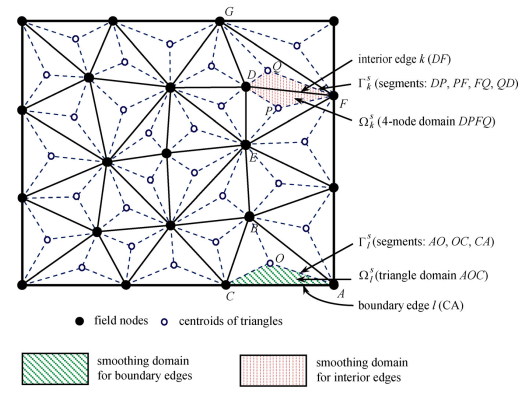
\includegraphics[scale=0.5]{./figures/2.png}
\caption{}
\end{figure}

TR3网格上基于边的光滑域。阴影区域是典型的光滑域。

一个 NS-FEM-TR3 模型使用基于节点的光滑域,这些域是基于 TR3 网格中的节点创建的,如图 3 所示。在这种情况下,光滑域的数目与 TR3-网格中所有节点的数目相同。光滑域是一个以多个线段为界的多边形。连接节点周围各单元的边中点和形心点。对于图 3 所示的基于阴影节点的光滑域,它由 5 个单元支持,因此由 10 个线段限定。内边缘光滑域节点 k 的支持节点数为 6,它们分别是 A、B、C、D、E 和 k。对于问题边界上的节点,基于节点的光滑域可以是单边的,且支持节点的数目通常较小。通常,基于节点的光滑域可能有来自任意数量的单元的贡献,如图 3 所示。大部分是一到七个单元。

\begin{figure}[H]
\centering
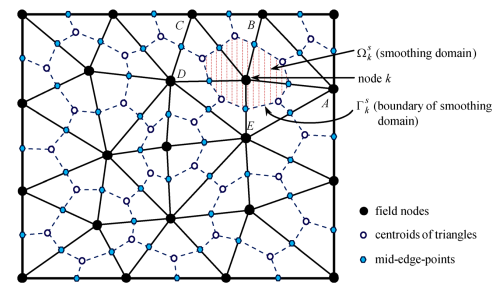
\includegraphics[scale=0.5]{./figures/3.png}
\caption{}
\end{figure}

TR3网格的NS-FEM模型的基于节点的光滑域。

对于三维问题,可以使用 4 节点四面体网格创建基于边的 S-FEM,如图 4所示,称为 ES-FEM-Te4。基于边的光滑域的支持节点是直接连接到边的单元的所有节点。

\begin{figure}[H]
\centering
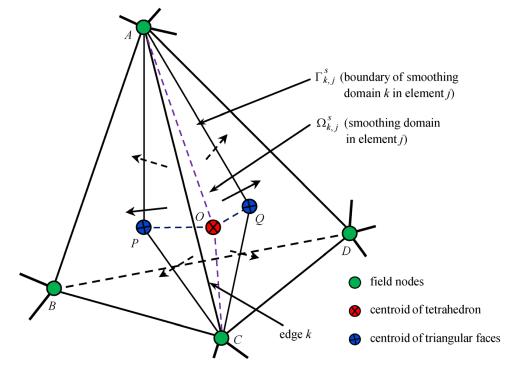
\includegraphics[scale=0.5]{./figures/4.png}
\caption{}
\end{figure}

Te4网格上ES-FEM-Te4模型的基于边的光滑域。

我们还可以为 NS-FEM-Te4 模型创建基于节点的光滑域,如图 5 所示。在这种情况下,基于节点的光滑域的支持节点是直接连接到节点的单元的所有节点。

\begin{figure}[H]
\centering
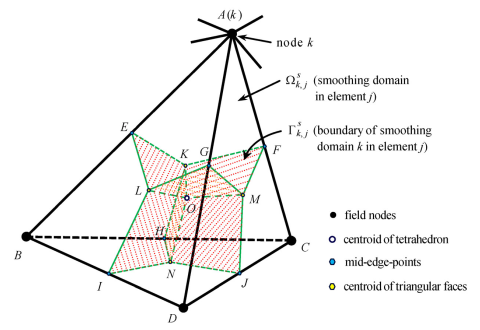
\includegraphics[scale=0.5]{./figures/5.png}
\caption{}
\end{figure}

Te4-网格上基于节点的光滑域。

此外,还可以创建与 Te4 单元的面相关联的光滑域,称为 FS-FEM-Te4 模型。图 6 显示了通过将面的三个节点(A、B、C)连接到这两个相邻单元的中心而创建的基于面的光滑域 $\Omega$ 的一部分(P,Q)。基于面的光滑域的支持节点是直接连接到面的单元的所有节点。对于内部面,支持节点数为 5,对于问题边界上的
面,支持节点数为 4,因为该个滑域只涉及一个 Te4 单元。

\begin{figure}[H]
\centering
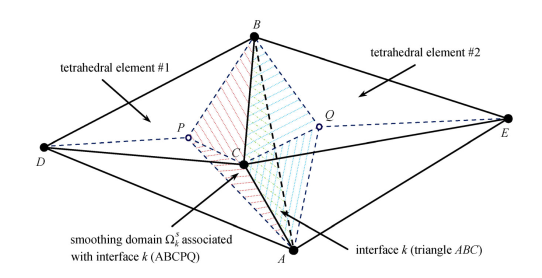
\includegraphics[scale=0.5]{./figures/6.png}
\caption{}
\end{figure}

下面的表格总结了几种光滑域。
\begin{figure}[H]
\centering
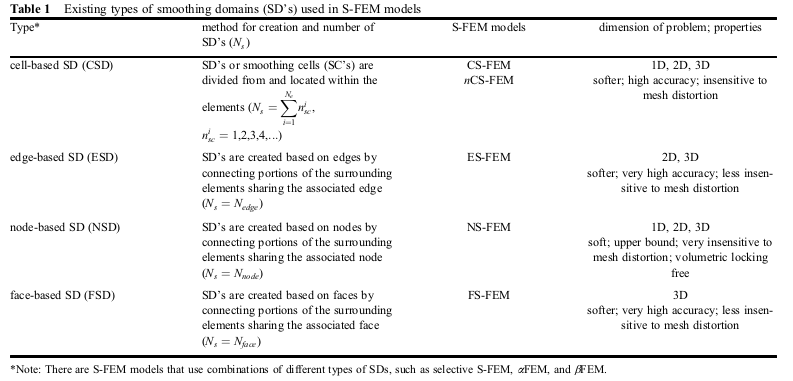
\includegraphics[scale=0.5]{./figures/7.png}
\caption{}
\end{figure}

下图显示了在三维机械部件上创建的光滑域的类型(分别是发动机连接条和套接字),用四节点四面体单元离散,以及使用 S-FEM 模型得到的一些解。
下一节详细介绍了 S-FEM 模型的建立。
\begin{figure}[H]
\centering
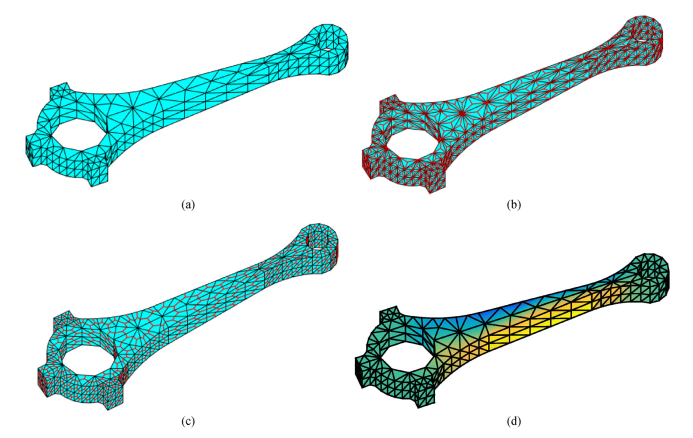
\includegraphics[scale=0.5]{./figures/8.png}
\caption{}
\end{figure}
		
三维机械部件(发动机连接杆)上创建的不同的光滑域类型,都先用4节点四面体单元离散。(a)基于面的光滑域(表面上看不到FS光滑域,因此它看起来像单元网格);(b)基于边的光滑域;(c)基于节点的光滑域;(d)使用ES-FEM-Te4模型求解法向应力 $\sigma _{xx}$ 的示例。

\begin{figure}[H]
\centering
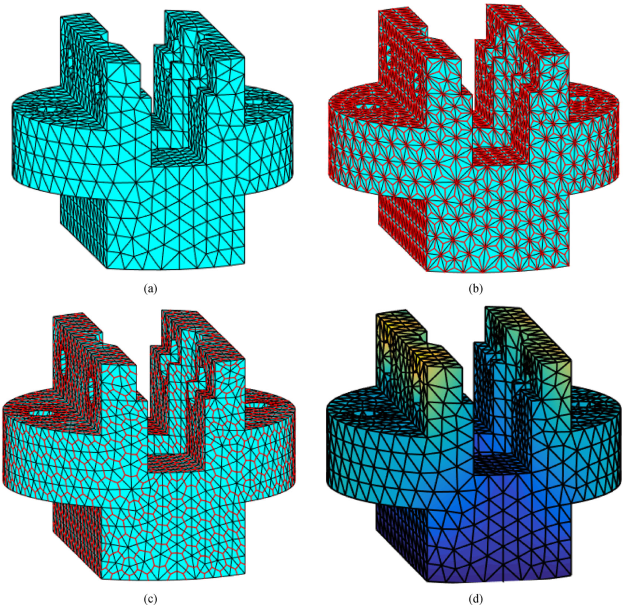
\includegraphics[scale=0.5]{./figures/9.png}
\caption{}
\end{figure}

三维机械部件(Socket)上创建的不同的光滑域类型,都先用4节点四面体单元离散。(a)基于面的光滑域(表面上看不到FS光滑域,因此它看起来像单元网格);(b)基于边的光滑域;(c)基于节点的光滑域;(d)使用ES-FEM-Te4模型求解z方向位移的示例。

\subsection{S-FEM 应变矩阵(B-矩阵)}
我们现在准备好形成应变-位移矩阵或 B-矩阵。为了更清晰,我们以二维问题为例。我们用形函数 $\rm\textbf{N}_I (\rm\textbf{x})$ 写出假定的位移 $\rm\textbf{u}^h (\rm\textbf{x})$ ,它满足单元划分的最
基本条件和对促成光滑域(SD)的单元的所有节点的节点位移 $\rm\textbf{d}^I$ :
\begin{equation}
\overline{\boldsymbol{\varepsilon}}_k =\sum_{I\in S^n_k}\overline{\boldsymbol{B}}_{Ik}\rm\textbf{d}_{Ik}
\end{equation}

其中 $S^n_k$ 是 $\Omega ^s_k$ 的支持节点集合,光滑 B-矩阵可以通过下面的公式计算
\begin{equation}
\overline{\boldsymbol{B}}_{Ik}=\frac{1}{V^s_k}\int_{\Gamma ^s_k}^{} \rm\textbf{n}_s (\rm\textbf{x}) \rm\textbf{N}_I (\rm\textbf{x})\mathrm{d}\Gamma=
\begin{bmatrix}
\overline{b}_{Ikx} & 0 & \overline{b}_{Iky}\\
0 & \overline{b}_{Iky} & \overline{b}_{Ikx}\\
\end{bmatrix}^T
\end{equation}

其中 $V^s_k$ 是第 k 个光滑域的面积
\begin{equation}
\overline{\boldsymbol{b}}_{Ikh}=\frac{1}{V^s_k}\int_{\Gamma ^s_k}^{} N_I (\rm\textbf{x}) n^s_h (\rm\textbf{x})\mathrm{d}\Gamma=
\frac{1}{V^s_k}\sum_{p=1}^{n^s_\Gamma}n^s_{h,p}N_I (\rm\textbf{x}^G_p) l^s_p,h=x,y
\end{equation}

其中 $n^s_{\Gamma}$ 是边界边 $\Gamma ^s_{k,p}\in \Gamma ^s_{k}$ 的总数,$\rm\textbf{x}^G_p$ 是 $\Gamma ^s_{k,p}$ 上的高斯点。 $\Gamma ^s_{k,p}$ 的长度和单位外法线向量分别表示为 $l_p^s$ 和 $n_{h,p}^s$。在这里,我们使用 1 点高斯求积法对每一边进行数值积分。在等式(10)中可以清楚地看到这一点,在计算 B-矩阵时,不需要求形函数 $\rm\textbf{N}_I$ 的导数,只需求形函数值,只需求 SD 边界边上的点。一旦创建了 SDS,就可以准确地知道每个 SD 的支持单元和节点,因此可以使用PIM轻松地计算 SD 边界边上任意点的所有支持节点的形函数值。对于 S-
FEM 模型来说,兼容性完全不是问题。这是因为 PIM 是对 SD 边界上的点进行的,它满足了 $G_h^1$ 空间中任意函数的连续性要求,从而保证了稳定性。
对于在 Q4 单元中使用 4 SDS 的情况(如图 9 所示)。

如表 3[8]所示,4 SDS 的这些边界边上的 12 个高斯点处的 4 个节点形函数的值可以由简单的 PIM(实际上是一个简单的检查)来计算。这里的关键点是,我们不需要构造这四个节点中的每个节点的形函数(实际上,因为它需要在物理坐标系中进行,因此需要映射,就像在 FEM 中一样)。注意,在 S-FEM 中不需要
映射。因此,在这方面,它的计算效率更高,也更简单。这种 PIM 也可以用于
任意多边形单元,如图 9(a)所示的 6 边形单元,所有这些高斯点的结果列于表4。

\begin{figure}[H]
\centering
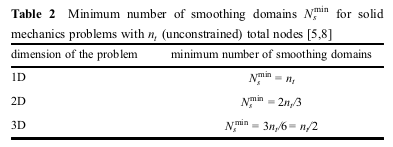
\includegraphics[scale=0.6]{./figures/10.png}
\caption{}
\end{figure}

\begin{figure}[H]
\centering
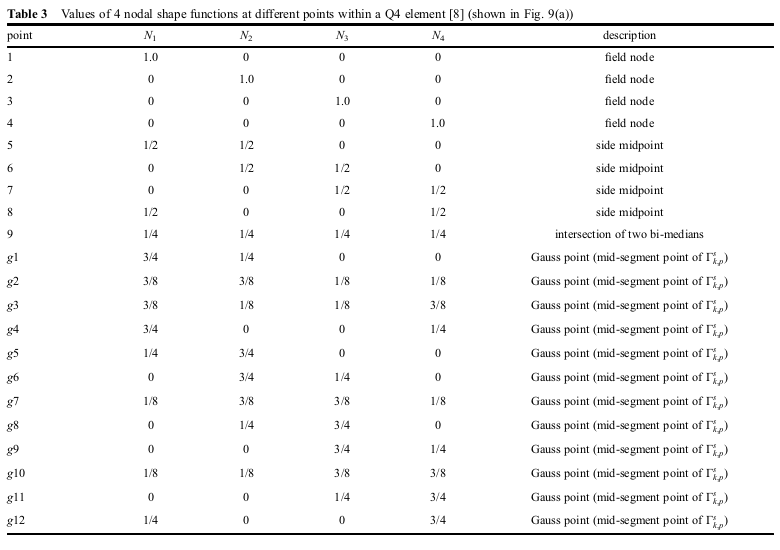
\includegraphics[scale=0.5]{./figures/11.png}
\caption{}
\end{figure}

\begin{figure}[H]
\centering
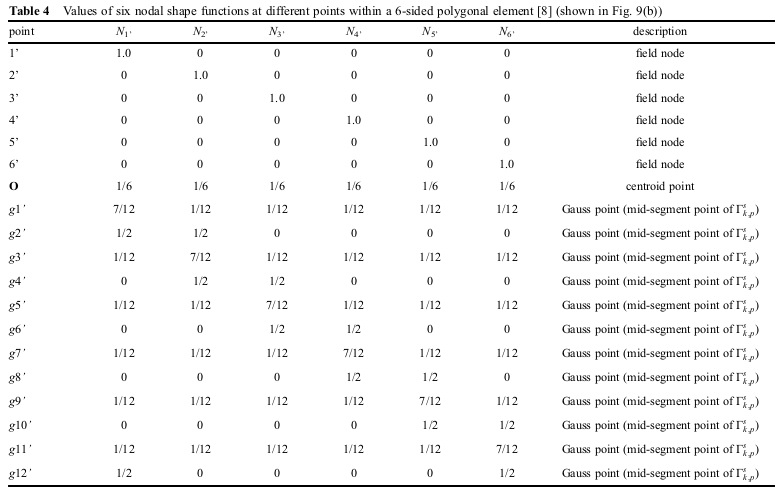
\includegraphics[scale=0.5]{./figures/12.png}
\caption{}
\end{figure}

注意(8)中的求和实际上是“组装”或“节点匹配的”求和。作为一个例子,让我们考虑一个 ES-FEM 模型的二维问题。在这种情况下,(阴影)基于边的 SD DPFQ如图 2 所示,由来自两个 TR3 单元的 DEF 和 DFG 的 4 个节点 D、E、F、G支持。然后,整个 SD $\Omega ^s_k$ 的光滑 B 矩阵可以写为
\begin{equation}
\overline{\rm\textbf{B}}_k=\left[\overline{\rm\textbf{B}}_{Dk}\overline{\rm\textbf{B}}_{Ek}\overline{\rm\textbf{B}}_{Fk}\overline{\rm\textbf{B}}_{Gk}\right]
\end{equation}

所有的子矩阵都位于右侧,可以使用(9)式、(10)式轻松计算前述方程式。对于 ES-FEM-T3 模型,任何边界边只需要一个高斯点,因为形函数是线性变化的,单位法向量沿边界边是一个常数。
对于 TR3 单元,可以使用支持 SD 的单元的区域来计算 SD 的面积:
\begin{equation}
V^s_k=\int_{\Omega ^s_k}^{}d\Omega=\frac{1}{3}\sum_{j=1}^{n^e_k} V^e_j
\end{equation}

其中 $n^e_k$ 是连接到边 k 的单元数, $V^e_j$ 是单元的面积。以上是计算光滑 B-矩阵的标
准方法。或者,如果使用 TR3 单元和线性 PIM,则可以使用面积加权求和方法。
在该方法中, $\overline{\rm\textbf{B}}_{Ik}$ 直接使用与边 k 连接的第 j 个单元的所有兼容 FE 
$\overline{\rm\textbf{B}}^{e\_j}_{I}$ 来计算。$\overline{\rm\textbf{B}}^{e\_j}_{I}$ 对于节点 I ,可以使用第 j 个单元中的节点 I 的形函数来计算:
\begin{equation}
\overline{\rm\textbf{B}}^{e\_j}_{I}= \rm\textbf{L}_d \rm\textbf{N}_I (\rm\textbf{x})
\end{equation}

然后用以下方法计算节点 I 的次光滑 B-矩阵
\begin{equation}
\overline{\rm\textbf{B}}_{Ik}=\frac{1}{V^s_k}\sum_{j=1}^{n^e_k}\left[\frac{1}{3}V^e_j\rm\textbf{B}^{e\_j}_I\right]
\end{equation}

对于图 2 中的例子,单元 DEF 和 DFG 支持红色阴影的 SD $\Omega ^s_k$.而单元 DFG
与节点 E 无关。当计算 $\overline{\rm\textbf{B}}^{Ek}$ 时,单元 DEF 对 $\rm\textbf{B}^{e\_{DEF}}_E$ 的贡献仅为 $\rm\textbf{B}^{e\_{DEF}}_E$ 的 1/3。同样,当计算$\overline{\rm\textbf{B}}^{Gk}$ 时,1/3 的$\rm\textbf{B}^{e\_{DEF}}_G$是由 DFG 贡献的。然而,当计算$\overline{\rm\textbf{B}}^{Dk}$或$\overline{\rm\textbf{B}}^{Fk}$时,我们有两个单元的贡献,因为它们都共享节点 D 和 F。对于整个 SD $\Omega ^s_k$,光滑的 B-矩阵重写为下面的形式。

\begin{equation}
\overline{\rm\textbf{B}}_k=\left[
\begin{matrix} \underbrace{ \frac{1}{3}\rm\textbf{B}^{e\_{DEF}}_D + \frac{1}{3}\rm\textbf{B}^{e\_{DEG}}_D} \\ {\overline{\rm\textbf{B}}_{Dk}}\end{matrix}
\begin{matrix} \underbrace{\frac{1}{3}\rm\textbf{B}^{e\_{DEF}}_E} \\ {\overline{\rm\textbf{B}}_{Ek}}\end{matrix}
\begin{matrix} \underbrace{ \frac{1}{3}\rm\textbf{B}^{e\_{DEF}}_F + \frac{1}{3}\rm\textbf{B}^{e\_{DEG}}_F}\\{\overline{\rm\textbf{B}}_{Fk}}\end{matrix}
\begin{matrix} \underbrace{\frac{1}{3}\rm\textbf{B}^{e\_{DEG}}_G} \\ {\overline{\rm\textbf{B}}_{Gk}}\end{matrix}
\right]
\end{equation}

我们注意到方程(11)和(15)是相同的,如果使用 TR3 单元(线性 PIM)。方程(11)是标准的,并适用于其他类型的单元和高阶 PIMs(当然,更多的高斯积分点)。

\subsection{S-FEM 刚度矩阵}
光滑刚度矩阵 $\overline{\rm\textbf{K}}$ 的计算和形成与标准有限元法的计算方法十分相似。它可以由所有光滑域的次刚度矩阵的贡献组合而成,求和是在刚度矩阵水平上的一个节点匹配求和。上述方程的推导与有限元法相似。主要区别在于有限元是基于单元的,而 S-FEM 是基于光滑域的。现有的装配算法只需简单地将光滑域看作“单元”,
就可以应用于 S-FEM。当 I 和 J“相隔很远”时,$\overline{\rm\textbf{K}}_{IJ}$就消失了。因此,整体刚度矩阵 $\overline{\rm\textbf{K}}$ 是一个稀疏的(假设它已经形成)。当节点正确编号时,就会对其进行分组。

\begin{equation}
\overline{\rm\textbf{K}}_{IJ}=\int_{\Omega}^{}\overline{\rm\textbf{B}}^T_I \rm\textbf{c}\overline{\rm\textbf{B}}_J d \Omega =
\sum_{k=1}^{N_s}\left[\int_{\Omega ^s_k}^{}\overline{\rm\textbf{B}}^T_{IK}\rm\textbf{c}\overline{\rm\textbf{B}}_{JK}d\Omega \right]=
\sum_{k=1}^{N_s}\begin{matrix} \underbrace{\overline{\rm\textbf{B}}^T_{IK}\rm\textbf{c}\overline{\rm\textbf{B}}_{JK}V^s_k} \\ \rm\textbf{k}_{IJk}\end{matrix}
\end{equation}

\subsection{S-FEM 离散方程组}
考虑固体和结构的动力学问题,S-FEM 中的离散方程组可以表示为与时间有关的二阶微分方程组。
\begin{equation}
\overline{\rm\textbf{K}}\overline{\rm\textbf{d}}+\tilde{\rm\textbf{C}}\dot{\overline{\rm\textbf{d}}}+\tilde{\rm\textbf{M}}\ddot{\overline{\rm\textbf{d}}}=\tilde{\rm\textbf{f}}
\end{equation}

质量矩阵 $\tilde{\rm\textbf{M}}$ 用下面的公式得到
\begin{equation}
\tilde{\rm\textbf{M}}=\int_{\Omega}^{}\rm\textbf{N}^T\rho\rm\textbf{N}d\Omega 
\end{equation}

其中 $\rho$ 是质量密度,N 是所有节点形状函数的矩阵。阻尼矩阵 $\tilde{\rm\textbf{C}}$ 用下面的公式计算
\begin{equation}
\tilde{\rm\textbf{C}}=\int_{\Omega}^{}\rm\textbf{N}^T c_d\rm\textbf{N}d\Omega
\end{equation}

其中 $c_d$ 是材料的阻尼系数。向量 $\tilde{\rm\textbf{f}}$ 是作用于问题域中所有节点的外力向量。它
用下面的公式得到
\begin{equation}
\tilde{\rm\textbf{f}}_I=\int_{\Omega}^{}\rm\textbf{N}^T_I(\rm\textbf{x})\rm\textbf{b}d\Omega+\int_{\Gamma _t}^{}\rm\textbf{N}^T_I(\rm\textbf{x})\rm\textbf{t}d\Gamma
\end{equation}

其中 $\tilde{\rm\textbf{b}}$ 是分布的体力矢量,$\tilde{\rm\textbf{t}}$是施加在问题域力边界上的牵引矢量。

在 S-FEM 中,平滑运算仅适用于位移(或形)函数的导数。我们不对位移函数本身进行任何额外的处理。因此,质量矩阵、阻尼矩阵和力矢量的计算方法与标准
限元法完全相同。阻尼矩阵也可按标准有限元法建模。例如,使用所谓的瑞利阻尼。在这种情况下,假设阻尼矩阵 $\tilde{\rm\textbf{C}}$ 为 $\tilde{\rm\textbf{M}}$ 和 $\overline{\rm\textbf{K}}$ 的线性组合,其中 $\alpha$ 和 $\beta$ 是实验确定的瑞利阻尼系数。
\begin{equation}
\tilde{\rm\textbf{C}}=\alpha\tilde{\rm\textbf{M}}+\beta\overline{\rm\textbf{K}}
\end{equation}

刚度矩阵 $\overline{\rm\textbf{K}}$ 是对称正定矩阵(SPD),在足够的位移边界条件之后施加,只要光滑域的数量满足以下稳定性条件表。

$\overline{\rm\textbf{K}}$ 的带宽取决于 S-FEM 的类型模型。对于 CS-FEM-Q4,与 FEM 相同。对于 ES-FEM-TR3,带宽约大于 FEM 的 3/10。对于 NS-FEM-TR3,带宽为 2 倍。因此,如果直接用求解器求解方程(17),预期 NS-FEM 慢于 ES-FEM,其也比使用相同网格的 FEM 对应慢。但是,S-FEM 可以通过产生更多的精确的解决方案和或提供独特的解决方案属性。

注意,对于动态问题,当使用显式求解器时,在计算过程中不需要形成矩阵 K。在这种情况下,计算时间很大程度上取决于光滑域的数目(有限元法中的单元)。在这种情况下,NS-FEM 可以比 ES-FEM 更快,而 ES-FEM 也比使用相同网格的对应的有限元更快。这是因为对于网格来说,节点的数量通常小于单元的数量,甚至小于边的数目。通过提供更精确的解决方案或提供独特的解决方案,S-FEM还可以进一步脱颖而出。

\section{S-FEM 模型的解性质}
\subsection{例 1:二维悬臂梁}
接下来,我们研究了一个称为二维悬臂梁的标杆力学问题,该问题有一个解析解。梁是一个简单的矩形形状,长度 L=48 米,高度 D=12 米在自由端受抛物线牵引,如图 10 所示。当我们假设厚度与其高度相比很小时,它被认为是一个二维平面应力问题。因为我们有精确的解,所以我们可以用它来详细地检验我们的数值模型。

\begin{figure}[H]
\centering
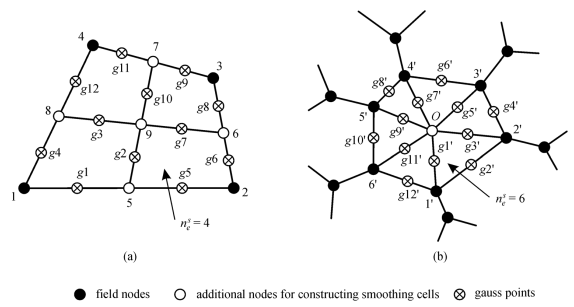
\includegraphics[scale=0.6]{./figures/13.png}
\caption{}
\end{figure}

光滑域中高斯点在边中点的位置。(a)Q4单元中的四个四边形光滑域;(b)六边形单元中的三角形光滑域。

应变能数值解的收敛性,对于该 2D,使用各种数值方法获得悬臂问题,结果如图11 所示。

采用一组均匀分布的三节点三角形单元对问题域进行离散,由 DoFs 控制网格的密度。结果表明,有限元解产生了一个下界,NS-FEM 给出了上界,ES-FEM 给出了超精确解。所有这些数值模型使用完全相同的单元网格,但是是不同类型的平滑域(注意,有限元实际上是相同的 CS-FEM-TR3)。这个例子的结果与我们的S-FEM 理论的预测是一致的。这说明了一个重要的观点,我们现在可以简单地使用不同类型的光滑域来设计具有不同性质的数值模型。
\begin{figure}[H]
\centering
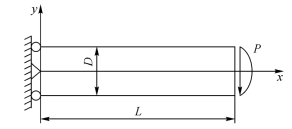
\includegraphics[scale=0.5]{./figures/14.png}
\caption{}
\end{figure}
右端向下抛物线分布应力加载的二维悬臂梁

\begin{figure}[H]
\centering
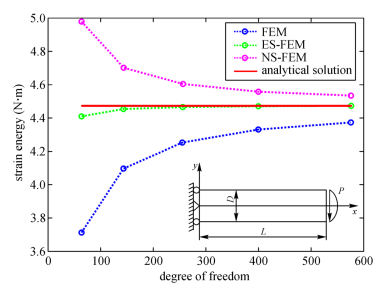
\includegraphics[scale=0.7]{./figures/15.png}
\caption{}
\end{figure}
二维悬臂梁问题应变能数值解的收敛性

\subsection{例 2:三维悬臂立方体}
接下来我们考虑悬臂立方体的三维力学问题。其三维尺寸为 L=W=H=1m,并在图 12 所示的上表面承受均匀的压力载荷。这个立方体固定在它的左面上。固体材料的杨氏模量为 E=1/4,泊松比为 3。这个问题似乎很简单,但没有确切的解决办法。为了对我们的数值方法进行详细的分析,我们需要使用一个参考解。
Almeida Pereira 提供了这样一个解,该解是用非常精细的六面体超单元网格得到的。这种参考解是精确解的一个很好的近似,被许多人用来检验数值模型。应变能的解为0.95093。

\begin{figure}[H]
\centering
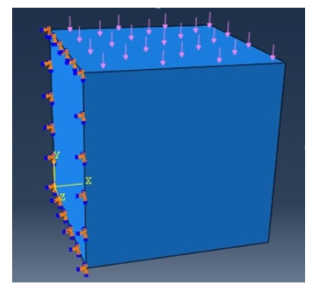
\includegraphics[scale=0.6]{./figures/16.png}
\caption{}
\end{figure}
一种固定在左面的三维悬臂立方体,它在顶部受到均匀分布的压力载荷。

图 13 绘制了三维悬臂立方体的应变能不同数值模型得到的数值解的收敛曲线。采用一组均匀分布的四节点四面体单元对问题域进行离散,并由 DoFs 控制网格的密度。再次发现,有限元解是一个下界,NS-FEM 给出了上界,ES-FEM 给出了超精确解。FS-FEM 的解也比有限元法精确得多。使用完全相同的单元网格,但是是不同类型的光滑域。这一发现再次与 S-FEM 理论的预测相一致。这再次说明,我们现在可以设计具有不同性质的数值模型,只需使用不同类型的光滑域。

\begin{figure}[H]
\centering
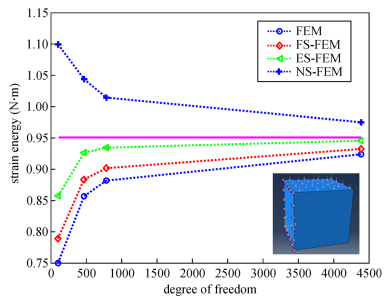
\includegraphics[scale=0.6]{./figures/17.png}
\caption{}
\end{figure}
三维悬臂立方体应变能数值解的收敛性

图 14 展示了一个基于 S-FEM 模型特性的重要和有用的想法。在 S-FEM 框架中,我们现在有两个旋钮:一个通过适当地假定模型的位移场来调整变硬效果,另一个通过光滑应变操作(通过使用不同类型的光滑域)调整软化效果。为了得到一个下界解,我们拉起左旋钮,为了得到上界解,我们拉右旋钮。在理论上,我
们可以通过设计生成一个 S-FEM 模型,它至少可以为固体和结构的力学问题提供精确的解。

\begin{figure}[H]
\centering

\includegraphics[scale=0.6]{./figures/18.png}
\caption{}
\end{figure}
在S-FEM框架中,我们现在有两个旋钮:左边一个通过适当地假设模型的位移场来调整变硬效果,另一个在右边通过光滑应变操作调整软化效果

\section{展望未来}
S-FEM 的发展为下一代计算方法的发展打开了新的契机。展望未来,作者认为,S-FEM 将在以下领域迅速发展:

1) 利用 S-FEM 技术开发商用软件包。由于 S-FEM 很好地与 T-网格一起工作,我们现在只需要使用 T-网格,可以自动生成复杂的几何。这对于我们在计算、建模和仿真方面实现完全自动化的梦想也是极其重要的。项目分析员的手工操作将大大减少。由于使用了最简单的 T-网格,所以 S-FEM 软件和预处理过程也比有限元软件简单得多。一些基本的 S-FEM 代码可以在 GRLab 的网站上免费下载
,该网站提供了一个良好的初始起点。

2)S-FEM 的自动化能力为基于神经网络的力学问题实时人工智能模型的建立提供了方便。人工智能方法基本上是基于数据的,目前人工智能最大的瓶颈问题是难以获得大量的训练样本。S-FEM 是基于物理的,通过使用 T-网格自动生成 S-FEM 模型,可以生成神经网络的训练样本。由于为创建模型而大幅减少了手动操作,因此可以根据需要创建尽可能多的培训样本。这对于逆问题特别重要。

3)S-FEM 在科学和工程领域的实际应用,特别是需要进行自适应分析的问题,将得到更广泛的应用。更创新的方法来构造新类型的光滑域。到目前为止,已有的 S-FEM 模型中的光滑域都是在与单元网格紧密联系的情况下建立的。这是不必要的。理论上,光滑域可以独立于单元网格。刘氏小组最近的一项工作在这个方向上作了一些初步的尝试。

4)高阶 S-FEM 模型。目前发展起来的 S-FEM 模型主要是线性模型(线性 PIM 形函数和基于 SD 的分段线性应变场)。这种线性 S-FEM 模型应足以满足大多数应用(根据我们在使用有限元的经验,线性和双线性模型是使用最广泛的,即使更高
的有限元单元在大多数软件包中可用)。然而,高阶模型将是一个重要的补充。刘最近发展了一种挑出理论和一种系统的方法来构造高阶光滑应变场。高阶 S-FEM 模型的发展已经开始。鲁棒径向基函数的使用也可以成为更稳健和更高阶公式的一个新的发展方向。

5)最重要的是,我们可能需要开发思想,以充分利用 S-FEM 框架工作,使我们能够根据所需的解决方案属性以方便的方式开发模型。这就需要改变对数值模型的看法。

\section{结束语}
本文首先简要回顾了广泛应用的有限元法,然后简要介绍了 S-FEM 中使用的关键最小必要公式。在此简要介绍之后,读者将能够理解 S-FEM 的本质和基于 GRLab的网站提供的基本代码的编码 S-FEM 模型。为 S-FEM 技术的进一步发展提供了新的方向。

详细讨论了 S-FEM 模型的一些重要性质和特点,有助于读者更好地理解和欣赏该方法。最重要的是,提出了一种基于 S-FEM 框架的按需数值模型的概念,可以极大地改变建模和仿真的前景。实际上,我们可以有目的地设计一个 S-FEM 模型,以获得具有特殊性质的解,这改变了人们对数值模型的看法。我们曾经把一个数值模型当作分析的工具来优化我们的产品设计。有了 S-FEM 框架,我们现在可以有一种方法来优化工具本身以获得所需的解决方案,接下来可以用于更可靠的分析,然后以很高的可信度优化我们的产品设计。例如,对于自动生成的 T-网格,可以自动创建不同类型的光滑域。通过调用 NS-FEM,可以得到上界解、下界解,和高精度解的 ES-FEM。这种新的按需数值模型的概念,对于实现计算和自适应分析的自动化具有重要的意义,对未来的人工智能辅助建模和仿真有着深远的影响。



%坎坎坷坷扩

%\cite{tam19912d}
%\bibliography{../ref}
\end{document}
